\chapter{Attention Mechanism (2014)}

\begin{tcolorbox}
\fullcite{arxiv/1409.0473/NMT-Jointly-Learning-Align-Translate}
\end{tcolorbox}


\section{Intro: Encoder-decoder \& Seq2seq}

\begin{enumerate}
    \item \textbf{Neural sequence modeling} is a framework in which a single neural network is trained end-to-end to map an input sequence to an output sequence. 
    \hfill \cite{arxiv/1409.0473/NMT-Jointly-Learning-Align-Translate, common/online/chatgpt}

    \item \textbf{Traditional models} often rely on \textbf{manually designed} intermediate representations or \textbf{fixed-length embeddings} that attempt to compress all input information into one vector. 
    This can create a bottleneck, since a single fixed-size representation may not capture all the necessary details of complex inputs. 
    \hfill \cite{arxiv/1409.0473/NMT-Jointly-Learning-Align-Translate, common/online/chatgpt}

    \item To overcome this limitation, we can allow the model to \textbf{dynamically focus on specific parts} of the input that are most relevant to generating each part of the output. 
    Instead of relying on a single static encoding, the model learns to compute \textbf{soft alignments}—that is, differentiable attention weights—over the input elements for each output step. 
    This enables the system to retrieve context \textbf{adaptively} and improve performance across diverse tasks.
    \hfill \cite{arxiv/1409.0473/NMT-Jointly-Learning-Align-Translate, common/online/chatgpt}

    \item Empirical results show that models with such attention mechanisms often outperform fixed-representation architectures, and the learned alignments correspond intuitively to which input regions influence particular outputs.
    \hfill \cite{arxiv/1409.0473/NMT-Jointly-Learning-Align-Translate, common/online/chatgpt}

    \item Many modern neural models for sequence or structured data processing follow an encoder–decoder architecture.
    The encoder processes the input data (e.g., a sequence, image, or signal) and compresses it into a single fixed-length representation. The decoder then uses this representation to generate or predict an output sequence.
    \hfill \cite{arxiv/1409.0473/NMT-Jointly-Learning-Align-Translate, common/online/chatgpt}
    \begin{enumerate}
        \item This encoder–decoder system is trained jointly so that the generated outputs are as accurate as possible given the inputs. 
        \hfill \cite{arxiv/1409.0473/NMT-Jointly-Learning-Align-Translate, common/online/chatgpt}
        
        \item A potential \textbf{limitation} of this setup is that it requires the entire input to be compressed into a single fixed-size vector. 
        This compression can lead to \textbf{information loss}, particularly for \textbf{long or complex inputs}. 
        As a result, performance tends to degrade when the input size or complexity increases, because the fixed-length representation cannot retain all relevant details.
        \hfill \cite{arxiv/1409.0473/NMT-Jointly-Learning-Align-Translate, common/online/chatgpt}
    \end{enumerate}

    \item To address the limitations of fixed-length representations, we extend the encoder–decoder framework by allowing the model to \textbf{jointly learn to focus and predict}.
    At each output step, the model dynamically determines which parts of the input are most relevant for generating the current output element.
    Instead of compressing the entire input into a single vector, the model performs a soft search over all input positions to identify where important information is concentrated.
    \hfill \cite{arxiv/1409.0473/NMT-Jointly-Learning-Align-Translate, common/online/chatgpt}

    \item Using these relevance scores (attention weights), the model computes a \textbf{context vector} as a weighted combination of the input representations.
    This context vector summarizes the most pertinent information for the current prediction and is used—along with information from previous outputs—to generate the next element in the output sequence.
    \hfill \cite{arxiv/1409.0473/NMT-Jointly-Learning-Align-Translate, common/online/chatgpt}

    \item The key advantage of this mechanism is that it \textbf{eliminates the fixed-size bottleneck} of traditional encoder–decoder models.
    By representing the input as a sequence (or set) of feature vectors and selecting among them adaptively, the model can handle inputs of arbitrary length and complexity without being forced to compress all information into one vector.
    This flexibility allows it to retain richer details and cope more effectively with long or information-dense inputs.
    \hfill \cite{arxiv/1409.0473/NMT-Jointly-Learning-Align-Translate, common/online/chatgpt}

    \item Empirical studies show that models trained to learn attention jointly with prediction achieve \textbf{significant performance improvements} compared to basic encoder–decoder models.
    Moreover, the learned attention weights often provide meaningful insight into how the model associates different parts of the input with particular outputs—demonstrating that the learned “alignments” reflect human-interpretable relevance patterns.
    \hfill \cite{arxiv/1409.0473/NMT-Jointly-Learning-Align-Translate, common/online/chatgpt}
\end{enumerate}




\section{Probabilistic Approach}

\begin{enumerate}
    \item From a probabilistic perspective, many learning tasks can be viewed as finding an output sequence $y$ that maximizes the \textbf{conditional probability} $P(y|x)$, where $x$ represents the input data.
    In practice, we train a parameterized model to approximate this conditional distribution using paired input–output data. 
    Once the conditional model is learned, predictions can be generated by selecting the output sequence that maximizes $P(y|x)$.
    \hfill \cite{arxiv/1409.0473/NMT-Jointly-Learning-Align-Translate, common/online/chatgpt}

    \item Recent advances have introduced \textbf{neural network–based approaches} to directly model this conditional distribution. 
    These approaches typically follow an \textbf{encoder–decoder design}: the encoder transforms the input $x$ into a learned internal representation, and the decoder generates the output $y$ conditioned on this representation.
    Recurrent neural networks (RNNs) or other sequential architectures (such as transformers or temporal CNNs) can be employed to handle variable-length inputs and outputs, encoding an input of arbitrary length into a fixed-length vector and then decoding it into a corresponding output sequence.
    \hfill \cite{arxiv/1409.0473/NMT-Jointly-Learning-Align-Translate, common/online/chatgpt}

    \item Although relatively new when first introduced, these neural encoder–decoder models demonstrated strong empirical performance on structured prediction tasks.
    For instance, recurrent architectures with memory mechanisms such as LSTMs were shown to achieve or surpass previous state-of-the-art results by capturing long-range dependencies between elements of the input and output.
    Further improvements were obtained by integrating neural sequence models with existing systems or by re-ranking candidate outputs using learned probabilistic scores.
    \hfill \cite{arxiv/1409.0473/NMT-Jointly-Learning-Align-Translate, common/online/chatgpt}
\end{enumerate}


\subsection{RNN Encoder-Decoder}


\begin{figure}[H]
    \centering
    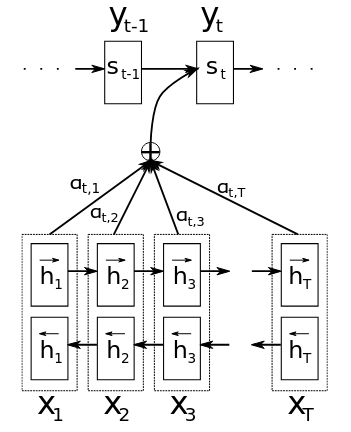
\includegraphics[
        width=\linewidth,
        height=5cm,
        keepaspectratio,
    ]{images/advanced-ml/arxiv-1409.0473v7.fig-1.model.png}
    \caption*{
        The graphical illustration of the proposed model trying to generate the $t$-th target token $y_t$ given a source sentence $(x_1, x_2, \cdots , x_T )$.
        \cite{arxiv/1409.0473/NMT-Jointly-Learning-Align-Translate, common/online/chatgpt}
    }
\end{figure}


\subsubsection*{Encoder}

\begin{enumerate}
    \item the encoder processes the input — represented as a sequence of vectors: $\bm{x}=(x_1,\cdots,x_{T_x})$ — and transforms it into an internal representation $c$.
    \hfill \cite{arxiv/1409.0473/NMT-Jointly-Learning-Align-Translate, common/online/chatgpt}

    \item A common implementation uses a recurrent neural network (RNN), where each hidden state $h_t$ is updated based on the current input and the previous hidden state: 
    \colorbox{yellow}{$h_t=f(x_t,h_{t-1})$}
    \hfill \cite{arxiv/1409.0473/NMT-Jointly-Learning-Align-Translate, common/online/chatgpt}

    \item The sequence of hidden states $\dCurlyBrac{h_1,\cdots,h_{T_x}}$ captures information about the entire input sequence.
    The final representation (or context vector) $c$ is then computed as a function of these hidden states: \colorbox{yellow}{$c=q(\dCurlyBrac{h_1,\cdots,h_{T_x}})$} 
    where $h_t \in \mbbR^n$ is a hidden state at time $t$, and $c$ is a vector generated from the sequence of the hidden states. 
    $f$ and $q$ are some nonlinear functions.
    \hfill \cite{arxiv/1409.0473/NMT-Jointly-Learning-Align-Translate, common/online/chatgpt}
    \begin{enumerate}
        \item LSTM can be used as $f$ and $q (\dCurlyBrac{h_1, \cdots , h_T }) = h_T$
        \hfill [Sutskever et al. (2014)] \cite{arxiv/1409.0473/NMT-Jointly-Learning-Align-Translate}
    \end{enumerate}

\end{enumerate}




\subsubsection*{Decoder}

\begin{enumerate}
    \item The decoder is often trained to predict the next token/token $y_{t^\prime}$ given the context vector $c$ and all the previously predicted tokens $\dCurlyBrac{y_1, \cdots , y_{t^\prime-1}}$.
    \hfill \cite{arxiv/1409.0473/NMT-Jointly-Learning-Align-Translate}

    \item In other tokens, the decoder defines a probability over the translation $\bm{y}$ by decomposing the joint probability into the ordered conditionals:
    \hfill \cite{arxiv/1409.0473/NMT-Jointly-Learning-Align-Translate}
    \\[0.2cm]
    .\hfill
    $
        p(\bm{y}) = \dprod_{t=1}^T P(y_t | \dCurlyBrac{y_1, \cdots , y_{t-1}} , c)
    $
    \hfill \cite{arxiv/1409.0473/NMT-Jointly-Learning-Align-Translate}
    \\[0.2cm]
    where $\bm{y} = (y_1, \cdots , y_{T_y})$.
    \hfill \cite{arxiv/1409.0473/NMT-Jointly-Learning-Align-Translate}

    \item With an RNN, each conditional probability is modeled as:
    \hfill \cite{arxiv/1409.0473/NMT-Jointly-Learning-Align-Translate}
    \\[0.2cm]
    .\hfill
    $ P(y_t | \dCurlyBrac{y_1, \cdots , y_{t-1}} , c) = g(y_{t-1}, s_t, c) $
    \hfill \cite{arxiv/1409.0473/NMT-Jointly-Learning-Align-Translate}
    \\[0.2cm]
    where $g$ is a nonlinear, potentially multi-layered, function that outputs the probability of $y_t$, and $s_t$ is the hidden state of the RNN.
    \hfill \cite{arxiv/1409.0473/NMT-Jointly-Learning-Align-Translate}

    \item Other architectures such as a hybrid of an RNN and a de-convolutional neural network can be used.
    \hfill \cite{arxiv/1409.0473/NMT-Jointly-Learning-Align-Translate}
\end{enumerate}









\section{Learning (RNN Encoder-Decoder)}

\subsection*{Encoder: Bidirectional RNN For Annotating Sequences}

\begin{enumerate}
    \item The usual RNN reads an input sequence $\bm{x}$ in order starting from the first symbol $x_1$ to the last one $x_{T_x }$. 
    However, we would like the annotation of each token to summarize not only the preceding tokens, but also the following tokens.
    \hfill \cite{arxiv/1409.0473/NMT-Jointly-Learning-Align-Translate}

    \item A BiRNN consists of forward and backward RNN’s. 
    The \textbf{forward RNN} $\overrightarrow{f}$ reads the input sequence as it is ordered (from $x_1$ to $x_{T_x}$ ) and calculates a sequence of forward hidden states $(\overrightarrow{h} _1, \cdots , \overrightarrow{h}_ {T_x} )$.
    The \textbf{backward RNN} $\overleftarrow{f}$ reads the sequence in the reverse order (from $x_{T_x}$ to $x_1$), resulting in a sequence of backward hidden states $(\overleftarrow{h} _1, \cdots , \overleftarrow{h} _{T_x} )$.
    \hfill \cite{arxiv/1409.0473/NMT-Jointly-Learning-Align-Translate}

    \item We obtain an annotation for each word xj by concatenating the forward hidden state $\overrightarrow{h}_ j$ and the backward one $\overleftarrow{h} _j $, i.e., $h_j = \dSquareBrac{\overrightarrow{h^\top}_ j ;\ \overleftarrow{h^\top}_ j}^\top$. 
    In this way, the annotation $h_j$ contains the summaries of both the preceding words and the following words. 
    Due to the tendency of RNNs to better represent recent inputs, the annotation $h_j$ will be focused on the words around $x_j $. 
    This sequence of annotations is used by the decoder and the alignment model later to compute the context vector $c_i$.
    \hfill \cite{arxiv/1409.0473/NMT-Jointly-Learning-Align-Translate}
\end{enumerate}




\subsection*{Decoder}

\begin{enumerate}
    \item we define each conditional probability as:
    $ P(y_i|y_1, \cdots , y_{i-1}, x) = g(y_{i-1}, s_i, c_i) $
    \hfill \cite{arxiv/1409.0473/NMT-Jointly-Learning-Align-Translate}
    \\[0.2cm]
    where $s_i$ is an RNN hidden state for time $i$, computed by 
    $s_i = f (s_{i-1}, y_{i-1}, c_i)$.
    \hfill \cite{arxiv/1409.0473/NMT-Jointly-Learning-Align-Translate}

    \item unlike the existing encoder–decoder approach ($p(\bm{y}) = \dprod_{t=1}^T P(y_t | \dCurlyBrac{y_1, \cdots , y_{t-1}} , c)$), here the probability is conditioned on a distinct context vector $c_i$ for each target token $y_i$.
    \hfill \cite{arxiv/1409.0473/NMT-Jointly-Learning-Align-Translate}

    \item The context vector $c_i$ depends on a sequence of annotations $(h_1, \cdots , h_{T_x} )$ to which an encoder maps the input sentence. 
    Each annotation $h_i$ contains information about the whole input sequence with a strong focus on the parts surrounding the $i$-th token of the input sequence. 
    \hfill \cite{arxiv/1409.0473/NMT-Jointly-Learning-Align-Translate}

    \item The context vector $c_i$ is, then, computed as a weighted sum of these annotations $h_i$:
    \hfill \cite{arxiv/1409.0473/NMT-Jointly-Learning-Align-Translate}
    \\[0.2cm]
    .\hfill
    $ ci = \dsum_{j=1}^{T_x} \alpha_{ij} h_j  $
    \hfill \cite{arxiv/1409.0473/NMT-Jointly-Learning-Align-Translate}

    \item The weight $\alpha_{ij}$ of each annotation $h_j$ is computed by:
    \hfill \cite{arxiv/1409.0473/NMT-Jointly-Learning-Align-Translate}
    \\[0.2cm]
    .\hfill
    $ \alpha_{ij}  =\dfrac{\exp (e_{ij} )}{\tsum_{k=1}^{T_x} \exp (e_{ik}) } $
    \hfill \cite{arxiv/1409.0473/NMT-Jointly-Learning-Align-Translate}
    \\[0.2cm]
    where \colorbox{yellow}{$e_{ij} = a(s_{i-1}, h_j )$} is an alignment model which scores how well the inputs around position $j$ and the output at position $i$ match. 
    The score is based on the RNN hidden state $s_{i-1}$ (just before emitting $y_i$, $ P(y_i|y_1, \cdots , y_{i-1}, x) = g(y_{i-1}, s_i, c_i) $) and the $j$-th annotation $h_j$ of the input sentence.
    \hfill \cite{arxiv/1409.0473/NMT-Jointly-Learning-Align-Translate}

    \item We parametrize the alignment model a as a feedforward neural network which is jointly trained with all the other components.
    The alignment is not considered to be a latent variable
    Instead, the alignment model directly computes a \textbf{soft alignment}, which allows the gradient of the cost function to be backpropagated through.
    This gradient can be used to train the alignment model as well as the whole translation model jointly.
    \hfill \cite{arxiv/1409.0473/NMT-Jointly-Learning-Align-Translate}

    \item We can understand the approach of taking a weighted sum of all the annotations as computing an \textbf{expected annotation}, where the expectation is over possible alignments. 
    Let $\alpha_{ij}$ be a probability that the target token $y_i$ is aligned to, or translated from, a source token $x_j $. 
    Then, the $i$-th context vector $c_i$ is the expected annotation over all the annotations with probabilities $\alpha_{ij} $.
    \hfill \cite{arxiv/1409.0473/NMT-Jointly-Learning-Align-Translate}

    \item The probability $\alpha_{ij} $, or its associated energy $e_{ij }$, reflects the importance of the annotation $h_j$ with respect to the previous hidden state $s_{i-1}$ in deciding the next state si and generating $y_i$. 
    Intuitively, this implements a mechanism of attention in the decoder.
    \hfill \cite{arxiv/1409.0473/NMT-Jointly-Learning-Align-Translate}
    
    \item The decoder decides parts of the source sentence to pay attention to. 
    By letting the decoder have an attention mechanism, we relieve the encoder from the burden of having to encode all information in the source sentence into a fixed-length vector. 
    With this new approach the information can be spread throughout the sequence of annotations, which can be selectively retrieved by the decoder accordingly.
    \hfill \cite{arxiv/1409.0473/NMT-Jointly-Learning-Align-Translate}

    \item An attention function can be described as \textbf{mapping a query} and a set of key-value pairs to an output, where the query, keys, values, and output are all vectors.
    \hfill \cite{arxiv/1706.03762/Attention-Is-All-You-Need}

    \item The output is computed as a \textbf{weighted sum} of the values, where the weight assigned to each value is computed by a compatibility function of the query with the corresponding key.
    \hfill \cite{arxiv/1706.03762/Attention-Is-All-You-Need}
\end{enumerate}














\section{How Attention Mechanism Works?}

\begin{enumerate}
    \item \textbf{Input Encoding}: Input data is transformed into a format that the model can process and creating representations of the data.
    \hfill \cite{geeksforgeeks/artificial-intelligence/ml-attention-mechanism/}

    \item \textbf{Query Generation}: A query vector is generated based on the current state or context of the model. 
    This query tells the model what it is looking for in the input data.
    \hfill \cite{geeksforgeeks/artificial-intelligence/ml-attention-mechanism/}

    \item \textbf{Key-Value Pair Creation}: Input is splitted into key-value pairs:
    \hfill \cite{geeksforgeeks/artificial-intelligence/ml-attention-mechanism/}
    \begin{enumerate}
        \item \textbf{Keys} represents the important information required to measure the relevant data.
        \hfill \cite{geeksforgeeks/artificial-intelligence/ml-attention-mechanism/}
        
        \item \textbf{Values} hold actual data.
        \hfill \cite{geeksforgeeks/artificial-intelligence/ml-attention-mechanism/}
    \end{enumerate}

    \item \textbf{Similarity Computation}: Model calculates similarity between the query vector and each key. This helps find how relevant each part of the input is. 
    Various methods can be used to calculate this similarity such as dot products or cosine similarity.
    \hfill \cite{geeksforgeeks/artificial-intelligence/ml-attention-mechanism/}
    \\[0.2cm]
    $
        \text{Score}(s,i) = 
        \begin{cases}
            h_s^{(1)}\cdot y_i & \text{ Dot Product} \\[0.2cm]
            (h_s^{(2)})^\top Wy_i & \text{ General} \\[0.2cm]
            v^\top \tanh\dParenBrac{W\dSquareBrac{\dfrac{h_s}{y_i}}} & \text{ Concat}
        \end{cases}
    $
    \hfill \cite{geeksforgeeks/artificial-intelligence/ml-attention-mechanism/}
    \\[0.2cm]
    \begin{enumerate}
        \item $h_s$: Encoder Source hidden state at position $s$
        \hfill \cite{geeksforgeeks/artificial-intelligence/ml-attention-mechanism/}

        \item $y_i$: Encoder Target hidden state at the position $i$
        \hfill \cite{geeksforgeeks/artificial-intelligence/ml-attention-mechanism/}

        \item $W$: Weight Matrix
        \hfill \cite{geeksforgeeks/artificial-intelligence/ml-attention-mechanism/}

        \item $v$: Weight vector
        \hfill \cite{geeksforgeeks/artificial-intelligence/ml-attention-mechanism/}
    \end{enumerate}
 
    \item \textbf{Attention Weights Calculation}: Similarity scores are passed through a softmax function to find attention weights. 
    These weights indicate the importance of each key-value pair.
    \hfill \cite{geeksforgeeks/artificial-intelligence/ml-attention-mechanism/}
    \\[0.2cm]
    .\hfill
    $\text{Attention Weight}(\alpha(s,i))=\text{softmax}(\text{Similarity Scores}(s,i))$
    \hfill \cite{geeksforgeeks/artificial-intelligence/ml-attention-mechanism/}

    \item \textbf{Weighted Sum}: Attention weights are applied to the corresponding values which helps in generating a weighted sum. 
    This step adds the relevant information from the input based on their importance calculated by the attention mechanism.
    \hfill \cite{geeksforgeeks/artificial-intelligence/ml-attention-mechanism/}
    \\[0.2cm]
    .\hfill
    $ c_t = \dsum^{T_s}_{i=1} \alpha(s,i)\ h_j^{(1)} $
    \hfill \cite{geeksforgeeks/artificial-intelligence/ml-attention-mechanism/}
    \\
    where $T_s$:  Total number of key-value pairs (source hidden states) in the encoder.
    \hfill \cite{geeksforgeeks/artificial-intelligence/ml-attention-mechanism/}

    \item \textbf{Context Vector}: Weighted sum act as a context vector which represents attended information from the input. It captures the relevant context for the current task. 
    \hfill \cite{geeksforgeeks/artificial-intelligence/ml-attention-mechanism/}

    \item \textbf{Integration with the Model}: Context vector is combined with the model's current state or hidden representation which provides additional information for other steps of the model.
    \hfill \cite{geeksforgeeks/artificial-intelligence/ml-attention-mechanism/}

    \item \textbf{Repeat}: Steps 2 to 8 are repeated for each step of the model which allows the attention mechanism to focus on different parts of the input sequence or data.
    \hfill \cite{geeksforgeeks/artificial-intelligence/ml-attention-mechanism/}
\end{enumerate}








\section{Self-Attention}

\begin{enumerate}
    \item Self-attention, sometimes called intra-attention is an attention mechanism relating different positions of a single sequence in order to compute a representation of the sequence. 
    \hfill \cite{arxiv/1706.03762/Attention-Is-All-You-Need}

    \item Self-attention has been used successfully in a variety of tasks including reading comprehension, abstractive summarization, textual entailment and learning task-independent sentence representation.
    \hfill \cite{arxiv/1706.03762/Attention-Is-All-You-Need}

    \item the self-attention mechanism allows every position to attend directly to every other position in a single step.
    \hfill \cite{common/online/chatgpt}

    \item That means any two tokens can interact in one operation, independent of how far apart they are in the sequence.
    \hfill \cite{common/online/chatgpt}

    \item the number of operations needed to connect two arbitrary positions is constant ($\mathcal{O}(1)$), not dependent on distance.
    \hfill \cite{common/online/chatgpt}

    \item Transformer is the first transduction model relying entirely on self-attention to compute representations of its input and output without using sequence-aligned RNNs or convolution. 
    \hfill \cite{arxiv/1706.03762/Attention-Is-All-You-Need}

    % \item 
\end{enumerate}





\section{Scaled Dot-Product Attention ($\text{Attention}(Q, K, V )$)}

\begin{figure}[H]
    \centering
    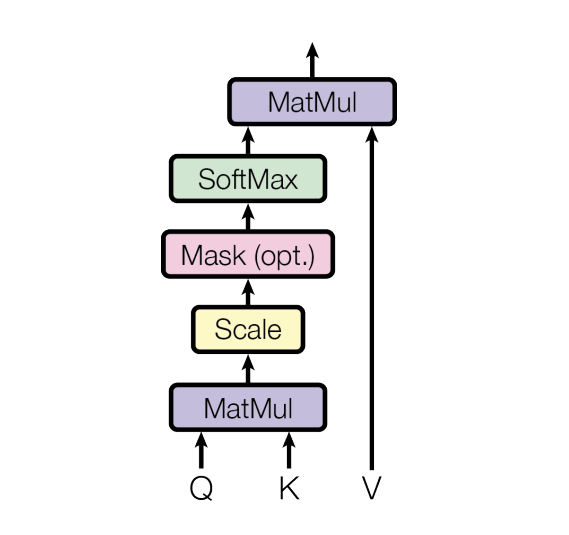
\includegraphics[
        width=\linewidth,
        height=7cm,
        keepaspectratio,
    ]{images/advanced-ml/Attention--Scaled-Dot-Product-Attention.png}
    \caption{Scaled Dot-Product Attention \cite{arxiv/1706.03762/Attention-Is-All-You-Need}}
\end{figure}


\begin{enumerate}
    \item The input consists of queries and keys of dimension $d_k$, and values of dimension $d_v$. 
    We compute the dot products of the query with all keys, divide each by $\sqrt{d_k}$, and apply a \textbf{softmax function} to obtain the weights on the values.
    \hfill \cite{arxiv/1706.03762/Attention-Is-All-You-Need}

    \item We compute the attention function on a set of queries simultaneously, packed together into a matrix $Q$. 
    The keys and values are also packed together into matrices $K$ and $V $. 
    We compute the matrix of outputs as:
    \hfill \cite{arxiv/1706.03762/Attention-Is-All-You-Need}
    \\[0.2cm]
    .\hfill
    $
        \text{Attention}(Q, K, V ) 
        = \text{softmax}\dParenBrac{\dfrac{QK^\top}{\sqrt{d_k}}}V
    $
    \hfill \cite{arxiv/1706.03762/Attention-Is-All-You-Need}

    \item The two most commonly used attention functions are additive attention, and dot-product (multiplicative) attention.
    \hfill \cite{arxiv/1706.03762/Attention-Is-All-You-Need}
    \begin{enumerate}
        \item Dot-product attention is identical, except for the scaling factor $\dfrac{1}{\sqrt{d_k}}$.
        \hfill \cite{arxiv/1706.03762/Attention-Is-All-You-Need}

        \item Additive attention computes the compatibility function using a feed-forward network with a single hidden layer.
        \hfill \cite{arxiv/1706.03762/Attention-Is-All-You-Need}
    \end{enumerate}
    While the two are similar in theoretical complexity, dot-product attention is much faster and more space-efficient in practice, since it can be implemented using highly optimized matrix multiplication code.
    \hfill \cite{arxiv/1706.03762/Attention-Is-All-You-Need}

    \item While for small values of $d_k$ the two mechanisms perform similarly, additive attention outperforms dot product attention without scaling for larger values of $d_k$ .
    We suspect that for large values of $d_k$, the dot products grow large in magnitude, pushing the softmax function into regions where it has extremely small gradients. 
    (To illustrate why the dot products get large, assume that the components of $q$ and $k$ are independent random variables with mean $0$ and variance $1$. 
    Then their dot product, $q \cdot k = \dsum^{d_k} _{i=1} q_ik_i$, has mean 0 and variance dk .)
    To counteract this effect, we scale the dot products by $\dfrac{1}{\sqrt{d_k}}$.
    \hfill \cite{arxiv/1706.03762/Attention-Is-All-You-Need}
\end{enumerate}









\section{Multi-Head Attention ($\text{MultiHead}(Q, K, V )$)}

\begin{figure}[H]
    \centering
    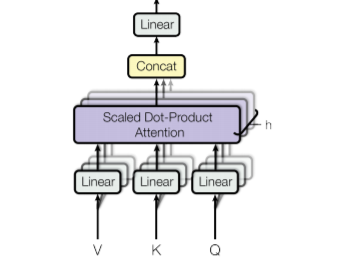
\includegraphics[
        width=\linewidth,
        height=7cm,
        keepaspectratio,
    ]{images/advanced-ml/Attention--Multihead-Attention.png}
    \caption{Multi-Head Attention \cite{arxiv/1706.03762/Attention-Is-All-You-Need}}
\end{figure}


\begin{enumerate}
    \item Instead of performing a single attention function with $d_{\text{model}}$-dimensional keys, values and queries, we found it beneficial to \textbf{linearly project} the queries, keys and values $h$ times with different, learned linear projections to $d_k$, $d_k$ and $d_v$ dimensions, respectively.
    \hfill \cite{arxiv/1706.03762/Attention-Is-All-You-Need}

    \item On each of these projected versions of queries, keys and values we then perform the attention function \textbf{in parallel}, yielding $d_v $-dimensional output values. 
    \hfill \cite{arxiv/1706.03762/Attention-Is-All-You-Need}
    
    \item These are concatenated and once again projected, resulting in the final values.
    \hfill \cite{arxiv/1706.03762/Attention-Is-All-You-Need}

    \item Multi-head attention allows the model to jointly attend to information from different representation subspaces at different positions. 
    With a single attention head, averaging inhibits this.
    \hfill \cite{arxiv/1706.03762/Attention-Is-All-You-Need}

    \item $ \text{MultiHead}(Q, K, V ) = \text{Concat}(\text{head}_1, \cdots, \text{head}_h)W^O $
    \hfill \cite{arxiv/1706.03762/Attention-Is-All-You-Need}
    \\[0.2cm]
    where $\text{head}_i = \text{Attention}(QW^Q_i , KW^K_i , V W^V_i )$, projections are parameter matrices $W^Q_i \in \mbbR^{d_{\text{model}}\times d_k} $, $W^K_i \in \mbbR^{d_{\text{model}}\times d_k} $, $W^V_ i \in \mbbR^{d_{\text{model}}\times d_v}$ and $W^ O \in \mbbR{hd_v \times d_{\text{model}}} $.
    \hfill \cite{arxiv/1706.03762/Attention-Is-All-You-Need}
\end{enumerate}























